\section{Verifying DaisyNFS}
\label{sec:proof}

A key contribution of DaisyNFS is a proof structure that isolates concurrency and crash
reasoning to the transaction system. This is done by giving GoTxn a specification
that captures how it enables sequential reasoning for the body of each
transaction, then carrying out that sequential reasoning in Dafny for the
DaisyNFS file-system logic. This section formalizes the theorem statements
involved in the proof, especially the transaction system's correctness theorem.

% How do we set up and prove the correctness of DaisyNFS?
%
The specification for \sys is a state-machine describing the ideal
version of \sys, namely that it appears to transition and respond
atomically according to the NFS state machine to all requests. The
implementation is a binary \cc{daisy-nfsd} that implements the NFS
protocol, running on top of a
disk. The \sys correctness
theorem is a \emph{refinement} property, which intuitively says that
for any interaction with the
implementation, the ideal, atomic specification could produce the responses;
this section shortly gives a more formal definition.
As a result a client interacting with the server can pretend
that it is the NFS state machine and ignore the complexities of its
implementation.

\begin{figure}[ht]
\small
\centering
\begin{tabular}{@{~}llr@{~}}
\toprule
\bf Layer & \bf Operations & \\
\midrule
  NFS
      & \cc{CREATE(d_ino, name)}, \cc{READDIR(d_ino)}, \dots & \cref{sec:spec} \\
  Txn
      & \cc{Read(tx, a, sz)}, \cc{Commit(tx)}, \cc{Alloc(a)},
        \dots & \cref{sec:system:txn} \\
  Disk
      & \cc{Read(a)}, \cc{Write(a, b)} & \\
\bottomrule
\end{tabular}
\caption{API layers of \sys.}
\label{fig:layers}
\end{figure}

The proof is about the server loop at three layers of abstraction, as outlined
in \cref{fig:layers}. The Disk layer at the bottom is where the whole server
runs, while the NFS layer serves as the specification. In addition, there
is an intermediate layer Txn for the transaction system which is the abstraction
on which the Dafny code is written and verified.

\tej{need to merge better text about GoTxn spec with the section in the GoTxn
chapter}

\resume

Now we have enough to state the final DaisyNFS correctness theorem:
\begin{theorem}[\sys correctness]
  $\mathrm{link}(\sdfy, \txncode) \refines \snfs$.%
  \label{thm:correctness}
\end{theorem}

\begin{figure}
  %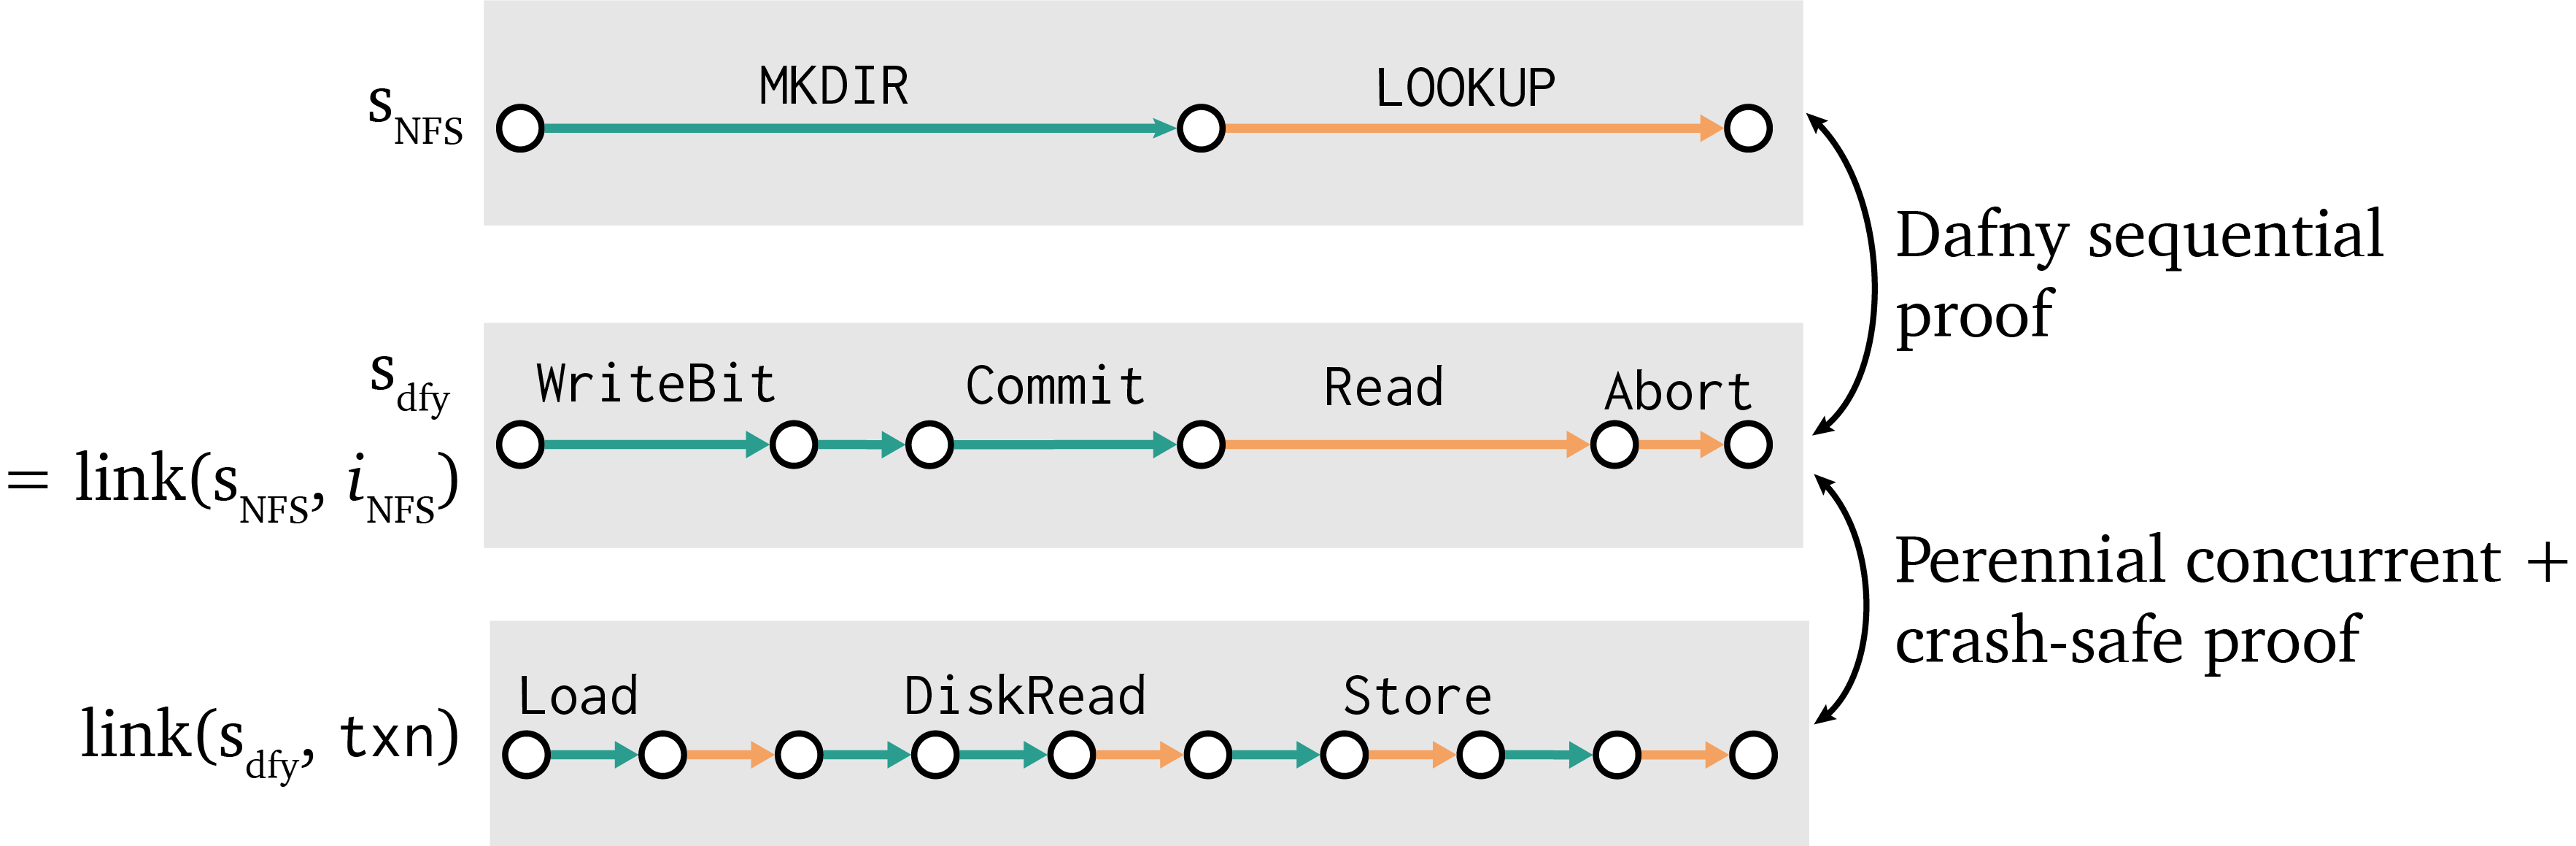
\includegraphics{fig/refinement-execs}
  \begin{center}
  \begin{tikzpicture}[scale=1, >=latex, every node/.append style={}]

  \tikzstyle{txnstate}=[circle,draw,minimum size=2mm,fill=blue!10]
  \tikzstyle{nfsstate}=[circle,draw,minimum size=2mm,fill=yellow!10]
  \tikzstyle{diskstate}=[circle,draw,minimum size=2mm,fill=green!10]
  \tikzstyle{switch}=[->, dashed, dash pattern=on 1.5pt off 2pt]
  \tikzstyle{stepr}=[thick,->]
  \tikzstyle{layer}=[font=\large]

  \setlength{\stepw}{1.25cm}
  \setlength{\dstepw}{\stepw*2}

  \newlength{\nfsbot}
  \newlength{\nfsmid}
  \setlength{\nfstop}{1.5cm}
  \setlength{\nfsbot}{.5cm}
  \setlength{\nfsmid}{(\nfstop+\nfsbot)/2}

  \newlength{\txntop}
  \newlength{\txnbot}
  \newlength{\txnmid}
  \setlength{\txntop}{-.5cm}
  \setlength{\txnbot}{-1.5cm}
  \setlength{\txnmid}{(\txntop+\txnbot)/2}

  \newlength{\disktop}
  \newlength{\diskbot}
  \newlength{\diskmid}
  \setlength{\disktop}{-2.5cm}
  \setlength{\diskbot}{-3.5cm}
  \setlength{\diskmid}{(\disktop+\diskbot)/2}

  \draw node (N0a) at (0,\nfstop) [nfsstate] {};
  \draw node (N1a) at (\dstepw,\nfstop) [nfsstate] {};
  \draw node (N1b) at (\dstepw,\nfsbot) [nfsstate] {};
  \draw node (N2b) at (\dstepw*2,\nfsbot) [nfsstate] {};

  \draw [stepr] (N0a.east) -- (N1a.west) node[midway,above=.2] {\code{LOOKUP}};
  \draw [stepr] (N1b.east) -- (N2b.west) node[midway,above=.2] {\code{CREATE}};
  \draw [switch] (N1a.south) -- (N1b.north);

  \draw node (T0a) at (0,\txntop) [txnstate] {};
  \draw node (T1a) at (\stepw,\txntop) [txnstate] {};
  \draw node (T2a) at (\stepw*2,\txntop) [txnstate] {};
  \draw node (T2b) at (\stepw*2,\txnbot) [txnstate] {};
  \draw node (T3b) at (\stepw*3,\txnbot) [txnstate] {};
  \draw node (T4b) at (\stepw*4,\txnbot) [txnstate] {};

  \draw [stepr] (T0a.east) -- (T1a.west) node[midway,above=.2] {};
  \draw [stepr] (T1a.east) -- (T2a.west) node[midway,above=.2] {\code{Commit}};
  \draw [switch] (T2a.south) -- (T2b.north);
  \draw [stepr] (T2b.east) -- (T3b.west) node[midway,above=.2] {};
  \draw [stepr] (T3b.east) -- (T4b.west) node[midway,above=.2] {\code{Abort}};

  \draw node (D0a) at (0,\disktop) [diskstate] {};
  \draw node (D1a) at (\stepw,\disktop) [diskstate] {};
  \draw node (D1b) at (\stepw,\diskbot) [diskstate] {};
  \draw node (D2b) at (\stepw*2,\diskbot) [diskstate] {};
  \draw node (D3b) at (\stepw*3,\diskbot) [diskstate] {};
  \draw node (D3a) at (\stepw*3,\disktop) [diskstate] {};
  \draw node (D4a) at (\stepw*4,\disktop) [diskstate] {};

  \draw [stepr] (D0a.east) -- (D1a.west) node[midway,above=.2] {\code{Read}};
  \draw [switch] (D1a.south) -- (D1b.north);
  \draw [stepr] (D1b.east) -- (D2b.west) node[midway,above=.2] {\code{Write}};
  \draw [stepr] (D2b.east) -- (D3b.west) node[midway,above=.2] {};
  \draw [switch] (D3b.north) -- (D3a.south);
  \draw [stepr] (D3a.east) -- (D4a.west) node[midway,above=.2] {};

  \draw [align=center] node (NFS) at (\stepw*5.5,\nfsmid) [layer] {$\snfs$ \\ \gooselayer{NFS}};
  \draw [align=center] node (Txn) at (\stepw*5.5,\txnmid) [layer] {$\sdfy$ \\ \gooselayer{Txn}};
  \draw [align=center] node (Disk) at (\stepw*5.5, \diskmid) [layer] {$\linkedcode$ \\ \gooselayer{Disk}};

\end{tikzpicture}

  \end{center}
  \vspace{-\baselineskip}
  \caption{One possible execution of DaisyNFS, receiving parallel LOOKUP and
    CREATE operations, at its three abstraction levels.
    Within an execution each row is a thread, and dashed arrows indicate
    context switches.
    The proof shows the bottom execution is equivalent to an atomic execution of
    each thread at
    the Txn layer~(in \cref{thm:gotxn}),
    and sequential reasoning shows each atomic sequence behaves according to the NFS
    specification~(in \cref{thm:dafny}).}
  \label{fig:refinement-execs}
\end{figure}

%
In this correctness theorem, initialization requires running a Dafny method on
an empty disk. Subsequently the system boots by first recovering the transaction
system, then restoring the file system. \Cref{thm:correctness} will follow
from the correctness of the transaction system combined with the results from
Dafny.

In order to use the GoTxn simulation transfer theorem, \cref{thm:gotxn-transfer} to obtain \cref{thm:correctness}, we need to
prove that DaisyNFS's implementation, $i_{NFS}$, satisfies the sequential refinement conditions. To do so, we define
$\seqrefinement_{\mathrm{dfy}}(i)$, an encoding of sequential refinement
using Dafny pre- and post-conditions (as illustrated in \cref{fig:refinement}), and prove that DaisyNFS
satisfies these conditions in Dafny. The crash refinement condition (3) is
straightforward; crashes have no effect in both the Txn layer and the NFS layers
because they do not have ephemeral state.

\begin{theorem} $\seqrefinement_{\mathrm{dfy}}(i_{NFS})$ holds.
  \label{thm:dafny}
\end{theorem}

\begin{figure}
  \centering
  \begin{subfigure}{0.25\textwidth}
    \begin{tikzpicture}[>=latex, every node/.append style={}]

  \tikzstyle{exspecstate}=[circle,draw, dashed,minimum size=2mm,fill=gray!20]
  \tikzstyle{specstate}=[circle,draw,minimum size=2mm,fill=gray!20]
  \tikzstyle{nfsstate}=[circle,draw,minimum size=2mm]
  \tikzstyle{sim}=[-]
  \tikzstyle{exsim}=[-, dashed]
  \tikzstyle{stepr}=[thick,->]
  \tikzstyle{exstepr}=[thick,->, dashed]

  \setlength{\stepw}{.75cm}
  \setlength{\dstepw}{\stepw*2}
  \setlength{\nfstop}{0cm}
  \newlength{\spectop}{1cm}
  \setlength{\spectop}{1cm}

  \draw node (N0) at (0,\nfstop) [nfsstate] {};
  \draw node (N1) at (\stepw,\nfstop) [nfsstate] {};
  \draw node (N2) at (\stepw*2,\nfstop) [nfsstate] {};
  \draw node (N3) at (\stepw*3,\nfstop) [nfsstate] {};

  \draw [stepr] (N0.east) -- (N1.west) node[midway] {};
  \draw [stepr] (N1.east) -- (N2.west) node[midway,below=.3] {\code{CREATE}};
  \draw [stepr] (N2.east) -- (N3.west) node[midway] {};

  \draw node (S0) at (0,\spectop) [specstate] {};
  \draw node (S1) at (\stepw*3,\spectop) [exspecstate] {};
  \draw [exstepr] (S0.east) -- (S1.west) node[midway, above=.2] {\code{nfs3create_spec}};

  \draw [sim] (S0.south) -- (N0.north) node[midway,left=.1] {$R$};
  \draw [exsim] (S1.south) -- (N3.north) node[midway,right=.1] {$R$};

\end{tikzpicture}

  %  \caption{Diagram view of sequential refinement.}%
  %  \label{fig:refinement:diagram}%
  \end{subfigure}~~~\vrule~~~~%
\begin{subfigure}{0.3\textwidth}
  {\small
\begin{verbatim}

method CREATE(d_ino: uint64,
              name: Bytes)
 returns (r: Result<Ino>)
 requires R(txn_disk, fs)
 ensures R(txn_disk, fs)
 ensures r.Ok? ==>
 nfs3create_spec(d_ino, name,
   old(fs), fs, r.v)
\end{verbatim}
}
  %\caption{Dafny encoding}%
  %\label{fig:refinement:dafny}
\end{subfigure}
  \caption{Illustration of $\seqrefinement(i_{NFS})$ (left) and its encoding
in Dafny $\seqrefinement_{\mathrm{dfy}}(i_{NFS})$ (right), for one particular operation.
In the diagram, the solid parts are assumed, and the
dashed parts must be shown to exist. The complete Dafny spec is more precise about
errors.}
  \label{fig:refinement}
\end{figure}

From here we can apply \cref{thm:gotxn} to \cref{thm:dafny} and
obtain \cref{thm:correctness}. \Cref{fig:refinement-execs} illustrates
just one execution that the theorem covers: the transaction system proof guarantees an
atomic execution while the sequential refinement guarantees the transactions
themselves are correct. There are two trusted assumptions needed for the
theorems to compose. First, $\seqrefinement_{\mathrm{dfy}}(i_{NFS})$ should imply
$\seqrefinement(i_{NFS})$. That is, the encoding of the refinement
conditions in Dafny must be correct, but also the semantics of the transaction
system operations modeled in Dafny must match the Coq proof. Second, every Dafny
transaction must be valid, meaning $\mathrm{safe}(i_{NFS}(op))$. The Dafny code
satisfies safety due to a simple syntactic check: the only mutable state in the
file-system Dafny class is the transaction system, so file-system operations
cannot make mutations other than through GoTxn.
% We have some
% confidence this holds due to a simple check over the Dafny code: the only
% mutable state in the Dafny class that implements the file system is the ghost
% variables and the transaction system, so it cannot make mutations other than
% through GoTxn (ghost variables cannot influence execution due to the design of
% Dafny).

% this was our old text explaining program refinement and linking
\begin{comment}

\subsection{Correctness theorem for the transaction system}
\label{sec:proof:txn}


\cc{Txn} layer semantics serves as the interface between the Perennial and Dafny
proofs.  It specifies that transactions are atomic in the sense that code
enclosed within a transaction \cc{Begin} and \cc{Commit} happens all at once (or
does nothing, if \cc{Abort} is executed), without interleaving of steps by other
threads.

We define the correctness of the transaction system's implementation as a
\emph{program refinement}.
To set up this specification, consider a program $p : \gooselayer{Txn}$ that
uses transactions.
To run $p$, it is combined with the transaction-system implementation, producing
a program $\mathrm{link}(p, \txncode) : \gooselayer{Disk}$ that can be run on
top of a disk.
Transactions in the linked program continue to have the expected atomic
behavior, so long as transaction code in $p$ follows certain restrictions, such
as not accessing shared state outside the journal system.  We write
$\mathrm{safe}(p)$ to mean $p$ is ``safe'' in the sense that it follows these restrictions.

% To connect this idealized semantics to the behavior of implementation, we define
% an

% At a high level of abstraction, the main difficulty is to give a specification
% for the transaction system, which we do in several steps:
%
% \begin{enumerate}
%   \item First, we define an arbitrary Go program running on top of
%         the transaction system. For reasons we will explain shortly we will use
%         $p : \gooselayer{Txn}$ for such a program. To run such a program it
%         first needs to be linked with the transaction system implementation,
%         producing a program denoted $\mathrm{link}(p, \txncode)$.
%   \item The second idea is to say what the semantics of a program
%         $p : \gooselayer{Txn}$ is. Transactions are atomic in this semantics in
%         that the whole transaction transitions at once, without interleaving
%         other threads. The program can issue reads and writes within a
%         transaction, and they follow a simple state machine.
%   \item The final idea is to define ``safe'' programs $\mathrm{safe}(p)$, those
%         that follow the restrictions of the transaction system. The
%         specification only applies to safe programs.
% \end{enumerate}

%With these specification ideas in place, what we prove in Coq is the following
%theorem:

The correctness of the transaction system is summarized by the following theorem:

\begin{theorem}
  The transaction system's implementation $\txncode$ is a program refinement, meaning for
  all $p : \gooselayer{Txn}$, if $\mathrm{safe}(p)$, then
  $\mathrm{link}(p, \txncode) \refines p$. The definition of
  $\mathrm{init}(\sigma_{s}, \sigma_{c})$ in this refinement relates an all-zero physical
  disk to an all-zero transactional disk of the same size.
  \label{thm:txn}
\end{theorem}

\cref{thm:txn} is stated in Coq and has a fully mechanized proof in Perennial.
What it says is that if a program is safe, the program linked with the
transaction system always behaves as if its transactions were atomically
accessing a transactional disk logically maintained by the transaction system.
The definition of safety formalized in Coq requires that code within a
transaction not access any shared memory outside of the transaction layer; other
than that, transactions are permitted to issue reads, writes, and do other
computation. Safety also requires that transactions follow the preconditions of
the \cc{Read} and \cc{Write} operations, which require a discipline of accessing
each object with a fixed size. Finally, safe programs can only \cc{Abort} or
\cc{Commit} a given transaction once. The notion of safe program will be
important when linking this proof with the Dafny proofs, since the transaction
system's proof only applies to a safe caller.

In the Coq development, \cref{thm:txn} uses Goose~\cite{chajed:goose-coqpl}
to translate the transaction system's Go implementation into a model in Coq that
Perennial supports.

\subsection{Correctness theorem for sequential file-system transactions}
\label{sec:proof:dafny}

The top-level file-system is a program denoted $\sdfy : \gooselayer{Txn}$
written against the transaction-system API, where this program models the
top-level dispatch loop that repeatedly accepts an NFS request and responds to
it in a separate thread. What we prove using Dafny is that this implementation
refines a more abstract dispatch loop $\snfs$ where the transitions atomically
follow the NFS transition system:

\begin{theorem}
  $\sdfy \refines \snfs$. To establish the init relation in this definition,
  the caller runs a dedicated method in Dafny that assumes an all-zero
  transaction system and establishes the invariant all other operations rely on
  (including recovery).
  \label{thm:dafny}
\end{theorem}

We prove this theorem in Dafny using a standard \emph{forward simulation}
technique.  Instead of directly reasoning about the $\sdfy$ concurrent program
(which is not possible in Dafny) we instead consider each of its handler methods
separately. Because transactions run atomically, it is sound to use Dafny's
sequential specifications in terms of pre- and post-conditions to reason about
an individual method. If every method satisfies a refinement obligation using a
common abstraction relation, we know that the entire program satisfies
refinement as defined above. This proof method of forward simulation is
so common that many systems verified in Dafny do not mention it, or treat
simulation and refinement synonymously.

Crash safety does add one interesting case to forward simulation. In general for
a sequential storage system, recovery should satisfy a specification that assumes
a \emph{crash invariant} that the whole system maintains at each intermediate
point and establishes the abstraction relation, with a new abstract state
consistent with the specification's crash behavior~\cite{chajed:argosy}. Due to
our transaction system we can make one simplification: on crash, the system will
satisfy the abstraction relation and not just a weaker crash invariant, since
operations are atomic; furthermore, the file system automatically maintains the
abstraction relation for crashes during recovery since recovery itself uses a
single transaction. Recovery must still do some work since the abstraction
relation held prior to the crash using in-memory state that has been lost. We
give the precise specification proven in Dafny in \cref{appendix:proof}, and
also argue how it fits into the forward simulation proof.

\subsection{Linking the transaction system and Dafny correctness theorems}
\label{sec:proof:linking}

Using the mechanized theorems, we can show that the overall system is correct,
namely that the running code implements the abstract NFS dispatch loop:

\begin{theorem}[\sys correctness]
  $\mathrm{link}(\sdfy, \txncode) \refines \snfs$. Initialization requires
  starting from an empty disk, then running the initialization implemented in
  Dafny. After that, the system boots by first recovering the transaction
  system's state, then running file-system recovery.
  \label{thm:correctness}
\end{theorem}

This theorem's proof is a straightforward consequence of the mechanized theorems
described as long as $\sdfy$ is safe; that is, the Dafny code follows the rules of
the transaction system. As long as this
holds we simply apply the theorems in order to show
$\mathrm{link}(\sdfy, \txncode) \refines \sdfy \refines \snfs$, since
the definition of refinement is transitive.

The proof requires Dafny operations to be encapsulated in transactions
and follow the transaction system's safety restrictions.
The code in Dafny does not generally manage starting and
committing a transaction; this is handled by a single wrapper function written
in Go. The wrapper creates a transaction, calls a Dafny method on it,
and then aborts if the method returns an error code and commits otherwise.
It is easy to confirm that this function follows the calling sequence required
by the transaction system.

Many transaction safety restrictions are preconditions on the
transaction-system APIs, which are enforced as Dafny preconditions.  The most
restrictive part of safety is that transactions are not allowed to read or write
shared memory, other than through the Txn layer. The Dafny code does allocate
heap objects and read them, but these are only used locally, and thus are
unaffected by concurrency; we work through this argument more formally in
\cref{appendix:proof}. To confirm that there is no shared mutable state, we
checked that the Dafny class implementing the file system has no mutable
variables, other than the transaction system and its allocators.  Dafny does not
support mutable global variables outside of any class, so checking the class is sufficient.

Notice that this linking proof makes minimal assumptions about the code in
Dafny, other than the fact that it is verified. In particular, the same argument
would equally apply to a different NFS implementation, or even a system with an
entirely different specification, as long as the equivalent of
\cref{thm:dafny} was still proven in Dafny, and the Dafny code did not use
shared mutable state.

% Formally, even if $\sdfy$ is not safe, it is sufficient if there
% exists any other program $\widetilde{\server}_{\mathrm{dfy}}$ with equivalent behavior which is
% safe; we can apply \cref{thm:txn} to this alternate program and get the same
% refinement result. Such a program would be a systematic transformation of the
% Dafny code that replaced any allocation with a local variable forwarded to the
% remainder of the code, and inlined any global constants. This transformation
% would could fail if Dafny wrote outside of its local allocations, but there are
% no mutable variables to write to. Finally, we manually check that any buffers
% returned from Dafny are used in a read-only manner.

The Txn layer's allocator methods are important for this approach to work.
The allocator cannot be implemented in Dafny because it is shared mutable state.
Instead, we expose the allocator API as part of a transaction, albeit with a loose
specification that says \cc{Alloc} may return
any number and \cc{Free} may be called on any unused block.
As we explain in \cref{sec:txn-proof}, under this specification, \cc{Alloc} and \cc{Free} both behave
atomically in a transaction. The
true allocation state is stored on disk, in the bitmap blocks for
example, and the Dafny code must validate that the address returned by \cc{Alloc} is actually
free.

% It is possible that one transaction calls
% \cc{Free} and another allocates the same number before the disk is updated,
% because freeing does not happen at commit time, but the allocator's policy is
% designed to delay allocating recently freed blocks so this is extremely
% unlikely.

\end{comment}
